\documentclass[a4paper, UTF8, zihao=-4]{ctexbook} %% CTeX宏集下的ctexbook文类,参数分别制定A4纸、源文件为UTF8编码格式,字号小四
\usepackage[Chinesetype=理学, Englishtype=Science, Chinesedegree=博士, Englishdegree=Doctor]{WUTthesis} %% 学位类别:理学(Science)、工学(Engineering)等,学位:硕士(Master)、博士(Doctor),其中理学博士为默认设置
\usepackage[backend=biber, maxbibnames=3, minbibnames=3, style=gb7714-2015, gbpub=false, gbnamefmt=lowercase]{biblatex} %% 文献处理宏包
\usepackage[colorlinks, linkcolor=blue, anchorcolor=red, citecolor=blue]{hyperref} %% 负责各种交叉引用的宏包
\usepackage{amssymb, amsfonts, amsmath, amsthm, mathtools} %% 和数学相关的一些宏包
\usepackage{listings} %% 关于代码抄录的宏包
\usepackage{multicol} %% 可以设置多列排版的宏包
\usepackage{graphicx} %% 和插图相关的宏包
\usepackage{txfonts, pxfonts} %% 数学字体宏包
\usepackage{upgreek} %% 数学字体宏包
\usepackage{mathrsfs} %% 数学字体红包
\usepackage{setspace} %% 调整行距的宏包
\usepackage{array} %% 制表宏包
\usepackage[usenames, dvipsnames]{xcolor} %% 颜色宏包
\usepackage{bigstrut} %% 该宏包提供 \bigstrut 命令,可以增大表格的行间距
\usepackage{titlesec}  %% A package providing an interface to sectioning commands for selection from various title styles. 
\usepackage[T1]{fontenc} %% 输出字体编码宏包,可选参数T1表明是T1编码
\usepackage{inputenc} %% 输入字体编码宏包
\usepackage{lmodern} %% 英文字体宏包 (Latin Modern Roman, Latin Modern Dunhill, Latin Modern Sans Serif, Latin Modern Sans Typewriter)
\usepackage{emptypage} %% 此宏包负责的任务是当每一章最后一页是偶数页时,设置空白
\usepackage[final]{pdfpages} %% 用于导入插入pdf文档的宏包




\renewcommand{\theequation}{\thechapter-\arabic{equation}} %% 将公式代号中默认的“.”改为“-”
\renewcommand{\thefigure}{\thechapter-\arabic{figure}} %% 将插图代号中默认的“.”改为“-”
\renewcommand{\thetable}{\thechapter-\arabic{table}} %% 将表格代号中默认的“.”改为“-”


\ctexset{chapter={format+={\zihao{-2}\heiti}, number={\arabic{chapter}}, afterskip={33pt}}} %% 设置章标题为字号小二,黑体,阿拉伯数字,章节标题与后面下方之间的距离为33pt
\ctexset{section={format+={\zihao{3}\heiti}, afterskip={21pt}}} %% 设置节标题为字号三号,黑体,阿拉伯数字,章节标题与后面下方之间的距离为22pt
\ctexset{subsection={format+={\zihao{4}\heiti}, afterskip={7pt}}} %% 设置小节标题为字号四号,黑体,阿拉伯数字,章节标题与后面下方之间的距离为7pt


\renewcommand{\bibfont}{\zihao{5}} %% 设置参考文献字号五号
\renewcommand{\bibauthorfont}{\bfseries\color{teal}} %% 设置参考文献中作者字段为粗体,蓝绿色
\renewcommand{\bibtitlefont}{\color{blue}} %% 设置参考文献中名称字段为蓝色
\renewcommand{\bibpubfont}{\itshape\color{violet}} %% 设置参考文献中出版项字段为斜体,紫色




\renewcommand{\lstlistingname}{代码} %% 设置代码抄录的标题名为”代码“
\lstset{basicstyle=\footnotesize\ttfamily, columns=fullflexible, numbers=left, numbersep=5pt, numberstyle=\tiny, backgroundcolor=\color{white}, frame=single, breaklines=true, showtabs=false, showspaces=false, showstringspaces=false, keywordstyle=\color{teal}, commentstyle=\color{blue}, stringstyle=\color{red}, numberstyle=\color{gray}, tabsize=8, breakatwhitespace=false, postbreak=\mbox{\textcolor{violet}{$\hookrightarrow$}\space}} %% 代码抄录的一系列设置
\AtBeginDocument{\renewcommand\thelstlisting{\ifnum \c@chapter>\z@ \thechapter-\fi \@arabic\c@lstlisting}} %% 将代码抄录代号中默认的“.”改为“-”





\setCJKfamilyfont{IPAMincho}{IPAMincho} %% 设置日文字体
\setCJKfamilyfont{IPAGothic}{IPAGothic} %% 设置日文字体
\setCJKfamilyfont{UnGungseo}{UnGungseo.ttf} %% 设置韩文字体
\setCJKfamilyfont{gulim}{gulim.ttf} %% 设置韩文字体
\newfontfamily\russian{DejaVu Serif} %% 设置俄文字体




\addbibresource{Bibliography.bib} %% 加入参考文献书库库文件



\begin{document}


\WUTclassificationnumber{} %% 分类号
\WUTconfidentiality{} %% 密级:只有涉密论文才填写
\WUTUDC{} %% UDC
\WUTuniversitycode{10497} %% 学校代码

\WUTChinesetitle{武汉理工大学研究生学位论文{\LaTeX}模板:\texttt{WUTthesis}} %% 论文中文题目
\WUTEnglishtitle{A {\LaTeX} Template for Writing Thesis by Postgraduates}{of Wuhan University of Technology: \texttt{WUTthesis}} %% 论文英文题目,由于一般英文题目过长,这里分成两行,所以这里相应地设置两个参数
\WUTauthor{顾加银}{Jiayin Gu} %% 论文作者:中文姓名,英文姓名
\WUTsupervisor{某某某}{XXX}{教授}{博士}{武汉理工大学}{430000} %% 指导教师:中文姓名、英文姓名、职称、学位、单位名称、邮编
\WUTvicesupervisor{on}{某某某}{教授}{博士}{武汉理工大学}{430000} %% 副指导教师:on/off (是否有,没有就在封面不显示)、姓名、职称、学位、单位名称、邮编
\WUTmajor{理论物理}{Theoretical Physics} %% 二级学科:中文专业名称、英文专业名称
\WUTinstitute{理学院} %% 院系名称
\WUTcommitteechairman{某某某} %% 答辩委员会主席
\WUTreviewers{某某某}{某某某} %% 评阅人
\WUTdegreeorganization{武汉理工大学} %% 学位授予单位
\WUTdates{2020年5月}{2020年5月}{2020年5月}{2020年6月}{May, 2020} %% 论文完成日期、论文完成日期、论文提交日期、论文答辩日期、学位授予日期、英文日期
\WUTdegreeabbreviation{Ph.D.} %% Ph.D. M.S. M.A.








\WUTmakefirstcover %% 生成封面一


\WUTmakesecondcover %% 生成封面二












 %% 插入封面文件
\begin{titlepage}


\mbox{}\vspace{5cm}

\begin{center}
\par \zihao{2}\kaishu 献给武汉理工大学!
\end{center}







\end{titlepage}
 %% 插入“献给XXX“的文件,此文件可有可无,不需要是删除或注释即可
\begin{titlepage}

\begin{adjustwidth}{6mm}{6mm}

\makebox[30mm]{\vspace{20mm}}

\begin{center}
\zihao{-2}\heiti 独创性声明
\end{center}
\vspace{5mm}
\begin{spacing}{1.4}
\par {\zihao{4}\STZhongsong  本人声明,所呈交的论文是本人在导师指导下进行的研究工作及取得的研究成果。尽我所知,除了文中特别加以标注和致谢的地方外,论文中不包含其他人已经发表或撰写过的研究成果,也不包含为获得武汉理工大学或其他教育机构的学位或证书而使用过的材料。与我一同工作的同志对本研究所做的任何贡献均已在论文中作了明确的说明并表示了谢意。}
\end{spacing}
\vspace{3mm}
\hspace{40mm}{\zihao{4}\STZhongsong 签\hspace{3mm}名:} \CJKunderline{\makebox[30mm]{}} \hspace{8mm} {\zihao{4}\STZhongsong 日\hspace{3mm}期:} \CJKunderline{\makebox[30mm]{}}


\vspace{40mm}




\begin{center}
\zihao{-2}\heiti 学位论文使用授权书
\end{center}
\vspace{3mm}
\begin{spacing}{1.4}
\par {\zihao{4}\STZhongsong 本人完全了解武汉理工大学有关保留、使用学位论文的规定,即学校有权保留并向国家有关部门或机构送交论文的复印件和电子版,允许论文被查阅和借阅。本人授权武汉理工大学可以将本学位论文的全部内容编入有关数据库进行检索,可以采用影印、缩印或其他复制手段保存或汇编本学位论文。同时授权经武汉理工大学认可的国家有关机构或论文数据库使用或收录本学位论文,并向社会公众提供信息服务。}
\end{spacing}
\vspace{3mm}
\hspace{53mm}{\zihao{4}\STZhongsong(保密的论文在解密后应遵守此规定)}

\vspace{20mm}
\noindent{\zihao{4}\STZhongsong 研究生(签名):} \hspace{20mm} {\zihao{4}\STZhongsong 导师(签名):} \hspace{20mm} {\zihao{4}\STZhongsong 日期:}


\end{adjustwidth}
\end{titlepage}



 %% 插入”独创性声明“文件






\frontmatter %% 开始前面部分,从此页码为罗马数字


\begin{WUTChineseabstract}
\par 本文是武汉理工大学研究生学位论文{\LaTeX}模板\texttt{WUTthesis}的文档。制作该模板,一来是为了让学位论文的撰写变得稍微容易一些,二来是为了借机宣传推广{\LaTeX}这个优秀的排版系统。\texttt{WUTthesis}由GitHub托管 \url{https://github.com/Jiayin-Gu/WUTthesis},并且采用了GNU GPLv3许可。
\end{WUTChineseabstract}
\WUTChinesekeywords{武汉理工大学,研究生,学位论文,{\LaTeX}模板}



















\begin{WUTEnglishabstract}
\par This is a documentation of the {\LaTeX} template \texttt{WUTthesis}, which is for writing thesis by postgraduates of Wuhan University of Technology. The template serves two purposes: one is to make thesis writing a little bit easier, and another is to advertise the excellent typeseting system {\LaTeX}. \texttt{WUTthesis} is hosted in GitHub \url{https://github.com/Jiayin-Gu/WUTthesis},and licensed with GNU GPLv3。
\end{WUTEnglishabstract}
\WUTEnglishkeywords{Wuhan University of Technology, Postgraduates, Thesis, {\LaTeX} Template}











\begin{spacing}{1.3} %% 可以适当调整spacing环境的参数,来控制目录的行距,以使得在必要的情况下将目录控制在两页之内
\tableofcontents     %% 目录
\end{spacing}




\mainmatter %% 开始主体部分,从此页码为阿拉伯数字


\def\path{Introduction}\chapter{引言}\label{chap_introduction}


\section{{\LaTeX}简介}


\begin{WUTquote}{Donald Kunth}
Microsoft Word is the last thing I want to use before I die.
\end{WUTquote}


\par {\LaTeX}是用于产生高品质文档的排版系统,而且事实上已经成为了学术出版的行业标准,国际上绝大多数学术期刊都要求接受{\LaTeX}稿件。{\LaTeX}排版系统基于的是“What you think is what you get.”(所思即所得)的思路\footnote{Microsoft Word、LibreOffice Writer、WPS Writer等排版软件基于的是“What you see is what you get.”(所见即所得)的思路。}。用于只需要关注文档的内容,而计算机会负责相关的格式处理。对于初学者有一定的难度,然而当熟练之后,{\LaTeX}便具有压倒性的优势,尤其是排版大型文档时,比如学位论文或书籍。{\LaTeX}的前身是1978年发布的{\TeX}排版系统,发明人为Donald Kunth教授(图~\ref{fig_Knuth})。1984年,Leslie Lamport博士编写了一组自定义命令宏包,取名LaTeX,该宏包对{\TeX}系统的若干命令进行了重新封装,使得整个排版系统使用起来方便了许多,并于次年发布了LaTeX宏包的源程序。逐渐的,{\TeX}排版系统也就演变为我们今天熟称的{\LaTeX}排版系统。{\LaTeX}是一个开源项目(\url{https://www.latex-project.org/}),世界各地的爱好者为{\LaTeX}系统编写了若干宏包,用于根据用户需求进行各式各样的格式处理,这些宏包及相关的说明文档可以从CTAN网站(Comprehensive {\TeX} Archive Network,\url{https://www.ctan.org/})下载。目前,国际上最大的{\TeX}/{\LaTeX}排版系统的用户组织为TUG(The TeX Users Group,\url{https://www.tug.org/})。关于{\LaTeX}的详细介绍,可以参考相关书籍\cite{Hu_2013, Liu_2013, Knuth_1986, Mittelbach_2004},或是相关的网络资料。



\begin{figure}
\begin{center}
\begin{minipage}[t]{0.7\hsize}
\resizebox{1.0\hsize}{!}{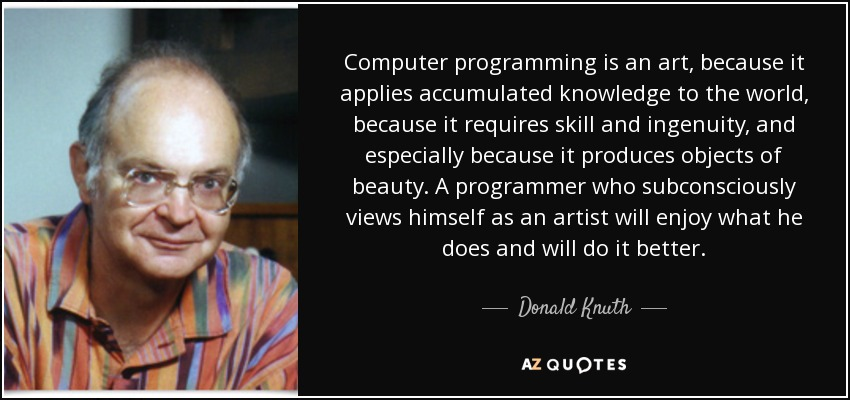
\includegraphics{\path/Knuth.jpg}}
\end{minipage}
\end{center}
\caption{{\TeX}系统的发明人Donald Kunth教授。}
\label{fig_Knuth}
\end{figure}







\section{\texttt{WUTthesis}}



\par 正由于{\LaTeX}在诸多方面的优势,国内越来越多的大学都开始鼓励采用其作为学位论文的排版系统,尤其是对于理工科专业。针对各大学学位论文的格式要求,一些校友们也已经制作了相应的学位论文{\LaTeX}模板。这里值得特别提出的是,在制作并推广学位论文{\LaTeX}模板方面,已经有两位武汉理工大学的校友作出过努力,他们的个人信息、作品名称,作品网址列出如下:
\begin{itemize}
\item 胡卫谊,2010年硕士研究生毕业,武汉理工大学计算机科学与技术学院,
\begin{itemize}
\item 作品:《武汉理工大学学位论文{\LaTeX}模板\texttt{WHUTthesis}》(研究生),
\item 作品网址:\url{https://code.google.com/archive/p/whutthesis/},
\item 作者邮箱:\texttt{whutthesis@gmail.com};
\end{itemize}
\item 曹宇,2015年本科毕业,武汉理工大学交通学院,
\begin{itemize}
\item 作品:《武汉理工本科论文{\LaTeX}模板》,
\item 作品网址:\url{https://github.com/tsaoyu/WHUT-LaTeX-bachelor},
\item 作者邮箱:\texttt{thesis@tsaoyu.com}。
\end{itemize}
\end{itemize}
但可惜的是,到目前位置(2020年2月),他们的工作并没有得到官方的认可,反而在提交学位论文进行反剽窃检查时,被要求提供doc格式的文档\footnote{此处省去太多吐槽。}。胡卫谊制作的模板因为长时间没有维护,再加上该模板在结构等方面存在一些需要改进和提升的地方,所以有必要重新制作新的模板,而本文就是针对这一目的介绍一种新的武汉理工大学研究生学位论文{\LaTeX}模板:\texttt{WUTthesis}。该新模板是根据《武汉理工大学博士、硕士学位论文撰写、印刷格式的统一要求(2009年7月修订)》制作的,模板在制作方面遵循一下原则:
\begin{itemize}
\item 模板要尽可能的简单,不做过多的封装,尽量将一些格式设置放在主文件的导言区。过多的封装会隐藏模板设计细节,从而影响用户对模板的理解。(这里鼓励用户在遵循学校统一格式要求和充分理解设计细节的情况下,根据自己的需求对模板进行修改。)
\item 模板的结构必须和学位论文的结构保持一致,从而可以使用户能快速且直观地理解模板的结构。
\end{itemize}


\par \texttt{WUTthesis}的改进和提升需要官方的配合,以及使用者的不断反馈。广大用户针对\texttt{WUTthesis}如果发现什么问题,或是有什么意见或建议,请联系作者本人,邮箱为\texttt{gujiayin1234@163.com}。{\color{red} 这里必须声明如下:由于\texttt{WUTthesis}格式上无法100\%地保证没有任何问题,再者,因为\texttt{WUTthesis}还未得到官方认可(到2020年2月为止),最终会要求在网上系统提交doc格式的文档,由此可能会引起的潜在种种问题,作者本人概不负责。}




\section{{\LaTeX}安装}

\par 下面列出一些{\LaTeX}套装以及相应的适用操作系统和官方网站
\begin{itemize}
\item MiKTeX (Microsoft Windows, \url{https://miktex.org/});
\item MacTeX (macOS, \url{https://www.tug.org/mactex/});
\item CTeX (Microsoft Windows, Chinese TeX, \url{http://www.ctex.org/HomePage})\footnote{这里需要区分CTeX套装和{\CTeX}宏集。};
\item TeX Live (Unix-like/Microsoft Windows/macOS, \url{http://tug.org/texlive/})。
\end{itemize}
如果在Ububtu(Linux的一种发行版)操作系统下,可以直接通过命令\texttt{sudo apt-get install texlive-full}安装。因为TeX Live具有最广泛的操作系统适用性,所以也自然成为最为推荐的{\LaTeX}套装,其相应的编辑器为 \href{http://www.tug.org/texworks/}{TeXworks}(Linux系统下需要单独安装并通过配置指定已安装的Tex Live可执行文件路径。)\footnote{TeXworks是一种开源的、跨平台、多语言支持的TeX/LaTeX编辑器。其他类似的编辑器包括 \href{https://www.texstudio.org/}{TeXstudio}、\href{https://www.xm1math.net/texmaker/}{Texmaker} 等。}。另外,需要指出的是,CTeX套装虽然针对中排版的{\LaTeX}系统,由于以下两个原因:
\begin{itemize}
\item 截止到2020年2月的最新版本,CTeX套装中并没有包含\texttt{biblatex-gb7714-2015}宏包(该宏包用于设置中文参考文献样式);
\item 其配套的WinEdt\footnote{\href{http://www.winedt.com/}{WinEdt} 是闭源软件,只适用与Microsoft Windows平台,不过用户可以免费使用该软件。}编辑器中并没有发现对应于\texttt{biblatex}宏包的参考文献处理程序\texttt{biber}按钮;
\end{itemize}
不建议使用。而实际上,由于上述原因,\texttt{WUTthesis}也未在CTeX套装上测试成功。不过新版CTeX套装预计会在2020年4月之前发布,变动会很大,我们拭目以待。当然,这里也鼓励喜欢钻研{\LaTeX}技术用户尝试解决上述两个原因造成的在使用\texttt{WUTthesis}过程出现的问题。

















 %% 导入第一章引言,Introduction为第一章文件夹名,\path 为对应的路径
\def\path{WUTthesis}\chapter{引言}\label{chap_introduction}


\section{{\LaTeX}简介}


\begin{WUTquote}{Donald Kunth}
Microsoft Word is the last thing I want to use before I die.
\end{WUTquote}


\par {\LaTeX}是用于产生高品质文档的排版系统,而且事实上已经成为了学术出版的行业标准,国际上绝大多数学术期刊都要求接受{\LaTeX}稿件。{\LaTeX}排版系统基于的是“What you think is what you get.”(所思即所得)的思路\footnote{Microsoft Word、LibreOffice Writer、WPS Writer等排版软件基于的是“What you see is what you get.”(所见即所得)的思路。}。用于只需要关注文档的内容,而计算机会负责相关的格式处理。对于初学者有一定的难度,然而当熟练之后,{\LaTeX}便具有压倒性的优势,尤其是排版大型文档时,比如学位论文或书籍。{\LaTeX}的前身是1978年发布的{\TeX}排版系统,发明人为Donald Kunth教授(图~\ref{fig_Knuth})。1984年,Leslie Lamport博士编写了一组自定义命令宏包,取名LaTeX,该宏包对{\TeX}系统的若干命令进行了重新封装,使得整个排版系统使用起来方便了许多,并于次年发布了LaTeX宏包的源程序。逐渐的,{\TeX}排版系统也就演变为我们今天熟称的{\LaTeX}排版系统。{\LaTeX}是一个开源项目(\url{https://www.latex-project.org/}),世界各地的爱好者为{\LaTeX}系统编写了若干宏包,用于根据用户需求进行各式各样的格式处理,这些宏包及相关的说明文档可以从CTAN网站(Comprehensive {\TeX} Archive Network,\url{https://www.ctan.org/})下载。目前,国际上最大的{\TeX}/{\LaTeX}排版系统的用户组织为TUG(The TeX Users Group,\url{https://www.tug.org/})。关于{\LaTeX}的详细介绍,可以参考相关书籍\cite{Hu_2013, Liu_2013, Knuth_1986, Mittelbach_2004},或是相关的网络资料。



\begin{figure}
\begin{center}
\begin{minipage}[t]{0.7\hsize}
\resizebox{1.0\hsize}{!}{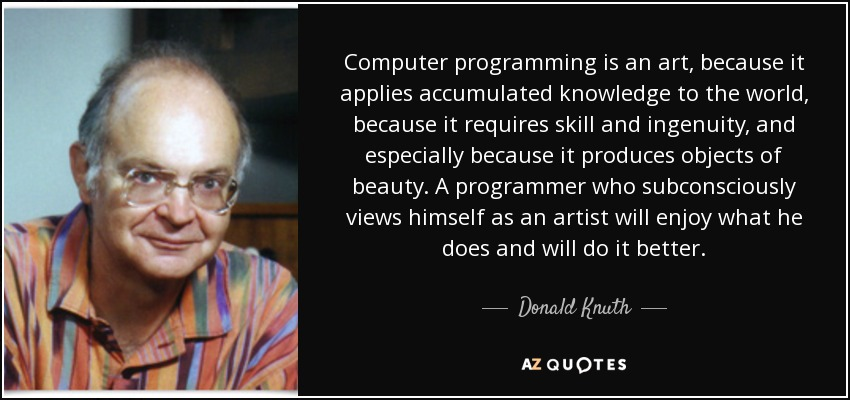
\includegraphics{\path/Knuth.jpg}}
\end{minipage}
\end{center}
\caption{{\TeX}系统的发明人Donald Kunth教授。}
\label{fig_Knuth}
\end{figure}







\section{\texttt{WUTthesis}}



\par 正由于{\LaTeX}在诸多方面的优势,国内越来越多的大学都开始鼓励采用其作为学位论文的排版系统,尤其是对于理工科专业。针对各大学学位论文的格式要求,一些校友们也已经制作了相应的学位论文{\LaTeX}模板。这里值得特别提出的是,在制作并推广学位论文{\LaTeX}模板方面,已经有两位武汉理工大学的校友作出过努力,他们的个人信息、作品名称,作品网址列出如下:
\begin{itemize}
\item 胡卫谊,2010年硕士研究生毕业,武汉理工大学计算机科学与技术学院,
\begin{itemize}
\item 作品:《武汉理工大学学位论文{\LaTeX}模板\texttt{WHUTthesis}》(研究生),
\item 作品网址:\url{https://code.google.com/archive/p/whutthesis/},
\item 作者邮箱:\texttt{whutthesis@gmail.com};
\end{itemize}
\item 曹宇,2015年本科毕业,武汉理工大学交通学院,
\begin{itemize}
\item 作品:《武汉理工本科论文{\LaTeX}模板》,
\item 作品网址:\url{https://github.com/tsaoyu/WHUT-LaTeX-bachelor},
\item 作者邮箱:\texttt{thesis@tsaoyu.com}。
\end{itemize}
\end{itemize}
但可惜的是,到目前位置(2020年2月),他们的工作并没有得到官方的认可,反而在提交学位论文进行反剽窃检查时,被要求提供doc格式的文档\footnote{此处省去太多吐槽。}。胡卫谊制作的模板因为长时间没有维护,再加上该模板在结构等方面存在一些需要改进和提升的地方,所以有必要重新制作新的模板,而本文就是针对这一目的介绍一种新的武汉理工大学研究生学位论文{\LaTeX}模板:\texttt{WUTthesis}。该新模板是根据《武汉理工大学博士、硕士学位论文撰写、印刷格式的统一要求(2009年7月修订)》制作的,模板在制作方面遵循一下原则:
\begin{itemize}
\item 模板要尽可能的简单,不做过多的封装,尽量将一些格式设置放在主文件的导言区。过多的封装会隐藏模板设计细节,从而影响用户对模板的理解。(这里鼓励用户在遵循学校统一格式要求和充分理解设计细节的情况下,根据自己的需求对模板进行修改。)
\item 模板的结构必须和学位论文的结构保持一致,从而可以使用户能快速且直观地理解模板的结构。
\end{itemize}


\par \texttt{WUTthesis}的改进和提升需要官方的配合,以及使用者的不断反馈。广大用户针对\texttt{WUTthesis}如果发现什么问题,或是有什么意见或建议,请联系作者本人,邮箱为\texttt{gujiayin1234@163.com}。{\color{red} 这里必须声明如下:由于\texttt{WUTthesis}格式上无法100\%地保证没有任何问题,再者,因为\texttt{WUTthesis}还未得到官方认可(到2020年2月为止),最终会要求在网上系统提交doc格式的文档,由此可能会引起的潜在种种问题,作者本人概不负责。}




\section{{\LaTeX}安装}

\par 下面列出一些{\LaTeX}套装以及相应的适用操作系统和官方网站
\begin{itemize}
\item MiKTeX (Microsoft Windows, \url{https://miktex.org/});
\item MacTeX (macOS, \url{https://www.tug.org/mactex/});
\item CTeX (Microsoft Windows, Chinese TeX, \url{http://www.ctex.org/HomePage})\footnote{这里需要区分CTeX套装和{\CTeX}宏集。};
\item TeX Live (Unix-like/Microsoft Windows/macOS, \url{http://tug.org/texlive/})。
\end{itemize}
如果在Ububtu(Linux的一种发行版)操作系统下,可以直接通过命令\texttt{sudo apt-get install texlive-full}安装。因为TeX Live具有最广泛的操作系统适用性,所以也自然成为最为推荐的{\LaTeX}套装,其相应的编辑器为 \href{http://www.tug.org/texworks/}{TeXworks}(Linux系统下需要单独安装并通过配置指定已安装的Tex Live可执行文件路径。)\footnote{TeXworks是一种开源的、跨平台、多语言支持的TeX/LaTeX编辑器。其他类似的编辑器包括 \href{https://www.texstudio.org/}{TeXstudio}、\href{https://www.xm1math.net/texmaker/}{Texmaker} 等。}。另外,需要指出的是,CTeX套装虽然针对中排版的{\LaTeX}系统,由于以下两个原因:
\begin{itemize}
\item 截止到2020年2月的最新版本,CTeX套装中并没有包含\texttt{biblatex-gb7714-2015}宏包(该宏包用于设置中文参考文献样式);
\item 其配套的WinEdt\footnote{\href{http://www.winedt.com/}{WinEdt} 是闭源软件,只适用与Microsoft Windows平台,不过用户可以免费使用该软件。}编辑器中并没有发现对应于\texttt{biblatex}宏包的参考文献处理程序\texttt{biber}按钮;
\end{itemize}
不建议使用。而实际上,由于上述原因,\texttt{WUTthesis}也未在CTeX套装上测试成功。不过新版CTeX套装预计会在2020年4月之前发布,变动会很大,我们拭目以待。当然,这里也鼓励喜欢钻研{\LaTeX}技术用户尝试解决上述两个原因造成的在使用\texttt{WUTthesis}过程出现的问题。


















\def\path{Conclusion_and_perspective}\chapter{引言}\label{chap_introduction}


\section{{\LaTeX}简介}


\begin{WUTquote}{Donald Kunth}
Microsoft Word is the last thing I want to use before I die.
\end{WUTquote}


\par {\LaTeX}是用于产生高品质文档的排版系统,而且事实上已经成为了学术出版的行业标准,国际上绝大多数学术期刊都要求接受{\LaTeX}稿件。{\LaTeX}排版系统基于的是“What you think is what you get.”(所思即所得)的思路\footnote{Microsoft Word、LibreOffice Writer、WPS Writer等排版软件基于的是“What you see is what you get.”(所见即所得)的思路。}。用于只需要关注文档的内容,而计算机会负责相关的格式处理。对于初学者有一定的难度,然而当熟练之后,{\LaTeX}便具有压倒性的优势,尤其是排版大型文档时,比如学位论文或书籍。{\LaTeX}的前身是1978年发布的{\TeX}排版系统,发明人为Donald Kunth教授(图~\ref{fig_Knuth})。1984年,Leslie Lamport博士编写了一组自定义命令宏包,取名LaTeX,该宏包对{\TeX}系统的若干命令进行了重新封装,使得整个排版系统使用起来方便了许多,并于次年发布了LaTeX宏包的源程序。逐渐的,{\TeX}排版系统也就演变为我们今天熟称的{\LaTeX}排版系统。{\LaTeX}是一个开源项目(\url{https://www.latex-project.org/}),世界各地的爱好者为{\LaTeX}系统编写了若干宏包,用于根据用户需求进行各式各样的格式处理,这些宏包及相关的说明文档可以从CTAN网站(Comprehensive {\TeX} Archive Network,\url{https://www.ctan.org/})下载。目前,国际上最大的{\TeX}/{\LaTeX}排版系统的用户组织为TUG(The TeX Users Group,\url{https://www.tug.org/})。关于{\LaTeX}的详细介绍,可以参考相关书籍\cite{Hu_2013, Liu_2013, Knuth_1986, Mittelbach_2004},或是相关的网络资料。



\begin{figure}
\begin{center}
\begin{minipage}[t]{0.7\hsize}
\resizebox{1.0\hsize}{!}{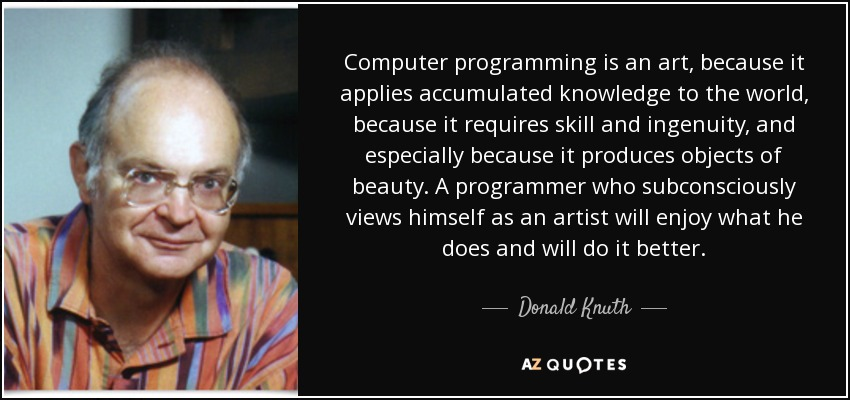
\includegraphics{\path/Knuth.jpg}}
\end{minipage}
\end{center}
\caption{{\TeX}系统的发明人Donald Kunth教授。}
\label{fig_Knuth}
\end{figure}







\section{\texttt{WUTthesis}}



\par 正由于{\LaTeX}在诸多方面的优势,国内越来越多的大学都开始鼓励采用其作为学位论文的排版系统,尤其是对于理工科专业。针对各大学学位论文的格式要求,一些校友们也已经制作了相应的学位论文{\LaTeX}模板。这里值得特别提出的是,在制作并推广学位论文{\LaTeX}模板方面,已经有两位武汉理工大学的校友作出过努力,他们的个人信息、作品名称,作品网址列出如下:
\begin{itemize}
\item 胡卫谊,2010年硕士研究生毕业,武汉理工大学计算机科学与技术学院,
\begin{itemize}
\item 作品:《武汉理工大学学位论文{\LaTeX}模板\texttt{WHUTthesis}》(研究生),
\item 作品网址:\url{https://code.google.com/archive/p/whutthesis/},
\item 作者邮箱:\texttt{whutthesis@gmail.com};
\end{itemize}
\item 曹宇,2015年本科毕业,武汉理工大学交通学院,
\begin{itemize}
\item 作品:《武汉理工本科论文{\LaTeX}模板》,
\item 作品网址:\url{https://github.com/tsaoyu/WHUT-LaTeX-bachelor},
\item 作者邮箱:\texttt{thesis@tsaoyu.com}。
\end{itemize}
\end{itemize}
但可惜的是,到目前位置(2020年2月),他们的工作并没有得到官方的认可,反而在提交学位论文进行反剽窃检查时,被要求提供doc格式的文档\footnote{此处省去太多吐槽。}。胡卫谊制作的模板因为长时间没有维护,再加上该模板在结构等方面存在一些需要改进和提升的地方,所以有必要重新制作新的模板,而本文就是针对这一目的介绍一种新的武汉理工大学研究生学位论文{\LaTeX}模板:\texttt{WUTthesis}。该新模板是根据《武汉理工大学博士、硕士学位论文撰写、印刷格式的统一要求(2009年7月修订)》制作的,模板在制作方面遵循一下原则:
\begin{itemize}
\item 模板要尽可能的简单,不做过多的封装,尽量将一些格式设置放在主文件的导言区。过多的封装会隐藏模板设计细节,从而影响用户对模板的理解。(这里鼓励用户在遵循学校统一格式要求和充分理解设计细节的情况下,根据自己的需求对模板进行修改。)
\item 模板的结构必须和学位论文的结构保持一致,从而可以使用户能快速且直观地理解模板的结构。
\end{itemize}


\par \texttt{WUTthesis}的改进和提升需要官方的配合,以及使用者的不断反馈。广大用户针对\texttt{WUTthesis}如果发现什么问题,或是有什么意见或建议,请联系作者本人,邮箱为\texttt{gujiayin1234@163.com}。{\color{red} 这里必须声明如下:由于\texttt{WUTthesis}格式上无法100\%地保证没有任何问题,再者,因为\texttt{WUTthesis}还未得到官方认可(到2020年2月为止),最终会要求在网上系统提交doc格式的文档,由此可能会引起的潜在种种问题,作者本人概不负责。}




\section{{\LaTeX}安装}

\par 下面列出一些{\LaTeX}套装以及相应的适用操作系统和官方网站
\begin{itemize}
\item MiKTeX (Microsoft Windows, \url{https://miktex.org/});
\item MacTeX (macOS, \url{https://www.tug.org/mactex/});
\item CTeX (Microsoft Windows, Chinese TeX, \url{http://www.ctex.org/HomePage})\footnote{这里需要区分CTeX套装和{\CTeX}宏集。};
\item TeX Live (Unix-like/Microsoft Windows/macOS, \url{http://tug.org/texlive/})。
\end{itemize}
如果在Ububtu(Linux的一种发行版)操作系统下,可以直接通过命令\texttt{sudo apt-get install texlive-full}安装。因为TeX Live具有最广泛的操作系统适用性,所以也自然成为最为推荐的{\LaTeX}套装,其相应的编辑器为 \href{http://www.tug.org/texworks/}{TeXworks}(Linux系统下需要单独安装并通过配置指定已安装的Tex Live可执行文件路径。)\footnote{TeXworks是一种开源的、跨平台、多语言支持的TeX/LaTeX编辑器。其他类似的编辑器包括 \href{https://www.texstudio.org/}{TeXstudio}、\href{https://www.xm1math.net/texmaker/}{Texmaker} 等。}。另外,需要指出的是,CTeX套装虽然针对中排版的{\LaTeX}系统,由于以下两个原因:
\begin{itemize}
\item 截止到2020年2月的最新版本,CTeX套装中并没有包含\texttt{biblatex-gb7714-2015}宏包(该宏包用于设置中文参考文献样式);
\item 其配套的WinEdt\footnote{\href{http://www.winedt.com/}{WinEdt} 是闭源软件,只适用与Microsoft Windows平台,不过用户可以免费使用该软件。}编辑器中并没有发现对应于\texttt{biblatex}宏包的参考文献处理程序\texttt{biber}按钮;
\end{itemize}
不建议使用。而实际上,由于上述原因,\texttt{WUTthesis}也未在CTeX套装上测试成功。不过新版CTeX套装预计会在2020年4月之前发布,变动会很大,我们拭目以待。当然,这里也鼓励喜欢钻研{\LaTeX}技术用户尝试解决上述两个原因造成的在使用\texttt{WUTthesis}过程出现的问题。


















\appendix\def\path{Appendices}

\chapter{\texttt{WUTthesis}日志}



\begin{itemize}
\item 2019年3月,作者本人使用{\LaTeX}排版博士学位论文,在此过程中依据学校规定的格式要求进行了大量的{\LaTeX}格式设置。在学校网上系统提交学位论文时有被要求提供doc格式文档,而作者本人将使用{\LaTeX}排版生成的pdf格式文档后缀名改为doc后提交,从而骗过了系统。
\item 2020年2月,作者本人根据去年在使用{\LaTeX}排版博士学位论文时进行大量格式设置制作了《武汉理工大学研究生学位论文{\LaTeX}模板:\texttt{WUTthesis}》,在Linux/Microsoft Windiows上基于TeX Live套装测试成功,同时将该模板发布到GitHub网站上。({\color{red}由于受COVID-19疫情的影响,几乎所有高校都推迟了春季开学时间,进而会耽误大量处于毕业季的研究生的正常毕业进度,这里希望\texttt{WUTthesis}能够在毕业生撰写学位论文过程中发挥点作用,至少减少一些因为调格式而产生的时间上的浪费。})
\end{itemize}








\chapter{{\LaTeX}工具箱}




\section{更多英文字体}
\par 表 \ref{tab_more_English_fonts} 列出更多英文字体,供用户根据实际需要使用。
\begin{table}
\caption{更多英文字体。}
\begin{center}
\begin{tabular}{>{\centering\arraybackslash}m{8.0cm}|>{\centering\arraybackslash}m{2.0cm}|>{\centering\arraybackslash}m{4.0cm}}
\hline
\hline
字体 & 字体码 & 示例 \bigstrut \\ \hline
Computer Modern Roman & \texttt{cmr} & {\fontfamily{cmr}\selectfont ABCDabcd1234} \bigstrut \\ \hline
Computer Modern Sans Serif & \texttt{cmss} & {\fontfamily{cmss}\selectfont ABCDabcd1234} \bigstrut \\ \hline
Computer Modern Typerwriter & \texttt{cmtt} & {\fontfamily{cmtt}\selectfont ABCDabcd1234} \bigstrut \\ \hline
Latin Modern Roman & \texttt{lmr} & {\fontfamily{lmr}\selectfont ABCDabcd1234} \bigstrut \\ \hline
Latin Modern Sans Serif & \texttt{lmss} & {\fontfamily{lmss}\selectfont ABCDabcd1234} \bigstrut \\ \hline
Latin Modern Sans Typerwriter & \texttt{lmtt} & {\fontfamily{lmtt}\selectfont ABCDabcd1234} \bigstrut \\ \hline
Latin Modern Dunhill & \texttt{lmdh} & {\fontfamily{lmdh}\selectfont ABCDabcd1234} \bigstrut \\ \hline
Times & \texttt{ptm} & {\fontfamily{ptm}\selectfont ABCDabcd1234} \bigstrut \\ \hline
Utopia/Fourier & \texttt{put} & {\fontfamily{put}\selectfont ABCDabcd1234} \bigstrut \\ \hline
Palatino & \texttt{ppl} & {\fontfamily{ppl}\selectfont ABCDabcd1234} \bigstrut \\ \hline
Pookman & \texttt{pbk} & {\fontfamily{pbk}\selectfont ABCDabcd1234} \bigstrut \\ \hline
Charter & \texttt{bch} & {\fontfamily{bch}\selectfont ABCDabcd1234} \bigstrut \\ \hline
Helvetica & \texttt{phv} & {\fontfamily{phv}\selectfont ABCDabcd1234} \bigstrut \\ \hline
Courier & \texttt{pcr} & {\fontfamily{pcr}\selectfont ABCDabcd1234} \bigstrut \\ \hline
{\TeX} Gyre Termes & \texttt{qtm} & {\fontfamily{qtm}\selectfont ABCDabcd1234} \bigstrut \\ \hline
{\TeX} Gyre Pagella & \texttt{qpl} & {\fontfamily{qpl}\selectfont ABCDabcd1234} \bigstrut \\ \hline
{\TeX} Gyre Bonum & \texttt{qbk} & {\fontfamily{qbk}\selectfont ABCDabcd1234} \bigstrut \\ \hline
{\TeX} Gyre Schola & \texttt{qcs} & {\fontfamily{qcs}\selectfont ABCDabcd1234} \bigstrut \\ \hline
{\TeX} Gyre Adventor & \texttt{qag} & {\fontfamily{qag}\selectfont ABCDabcd1234} \bigstrut \\ \hline
{\TeX} Gyre Heros & \texttt{qhv} & {\fontfamily{qhv}\selectfont ABCDabcd1234} \bigstrut \\ \hline
{\TeX} Gyre Cursor & \texttt{qcr} & {\fontfamily{qcr}\selectfont ABCDabcd1234} \bigstrut \\ \hline
\hline
\end{tabular}
\end{center}
\label{tab_more_English_fonts}
\end{table}

\section{一些西欧字符的输入}
\par 由于源文件采用的UTF8编码方式,所以一些带修饰的西欧字符可以直接输入,然而这对于长期习惯于英文输入的用户来说,可能会有一些困难。下面列出一些通过命令的方式来产生一些带修饰的字符:
\begin{itemize}
\item \verb"\`a", \`a;
\item \verb"\'e", \'e;
\item \verb"\""o, \"o;
\item \verb"\^u", \^u;
\item \verb"\c{c}", \c{c};
\item \verb"\v{Z}", \v{Z}。
\end{itemize}






\section{数学符号}

\begin{table}
\caption{Other Builtin Mathematical Relations, Operators, Symbols, Decorations, and Expressions in {\LaTeX}}
\begin{center}
\begin{tabular}{|c|c|c|c|c|c|} \hline
\verb"\Delta"  & $\Delta$ & \verb"\div" & $\div$ & \verb"\times" & $\times$ \bigstrut \\ \hline
\verb"\lim" & $\lim$ & \verb"\infty"  & $\infty$ & \verb"\sqrt{a}" & $\sqrt{a}$ \bigstrut \\ \hline
\verb"\frac{a}{b}" & $\frac{a}{b}$ & \verb"\infty" & $\infty$ & \verb"\circ"  & $\circ$ \bigstrut \\ \hline
\verb"\equiv" & $\equiv$ & \verb"\pm" & $\pm$ & \verb"{\rm text}" & ${\rm text}$  \bigstrut \\ \hline
\verb"\mp"  & $\mp$ & \verb"\star" & $\star$ & \verb"\sim" & $\sim$ \bigstrut \\ \hline
\verb"\simeq" & $\simeq$ & \verb"\approx"  & $\approx$ & \verb"\mp" & $\mp$ \bigstrut \\ \hline
\verb"\codt" & $\cdot$ & \verb"\partial" & $\partial$ & \verb"\doteq"  & $\doteq$ \bigstrut \\ \hline
\verb"\cong" & $\cong$ & \verb"\parallel" & $\parallel$ & \verb"\perp" & $\perp$  \bigstrut \\ \hline
\verb"\oint"  & $\oint$ & \verb"\nabla" & $\nabla$ & \verb"\int" & $\int$ \bigstrut \\ \hline
\verb"\Box" & $\Box$ & \verb"\propto"  & $\propto$ & \verb"\sum" & $\sum$ \bigstrut \\ \hline
\verb"\hbar" & $\hbar$ & \verb"\dagger" & $\dagger$  & \verb"\forall"  & $\forall$ \bigstrut \\ \hline
\verb"\exists" & $\exists$ & \verb"\uparrow" & $\uparrow$ & \verb"\downarrow" & $\downarrow$  \bigstrut \\ \hline
\verb"\neq"  & $\neq$ & \verb"\leq" & $\leq$ & \verb"\geq" & $\geq$ \bigstrut \\ \hline
\verb"\rightarrow" & $\rightarrow$  & \verb"\Rightarrow"  & $\Rightarrow$ & \verb"\Lefrightarrow" & $\Leftrightarrow$ \bigstrut \\ \hline
\verb"\in" & $\in$ & \verb"\to" & $\to$ & \verb"\gg"  & $\gg$ \bigstrut \\ \hline
\verb"\circleddot" & $\circleddot$ & \verb"\ll" & $\ll$ & \verb"\prod" & $\prod$  \bigstrut \\ \hline
\verb"\langle"  & $\langle$ & \verb"\rangle" & $\rangle$ & \verb"\angle" & $\rangle$ \bigstrut \\ \hline
\verb"\prime" & $\prime$  & \verb"\wedge"  & $\wedge$ & \verb"\slash" & $\slash$ \bigstrut \\ \hline
\verb"{\boldsymbol\lambda}" & ${\boldsymbol\lambda}$ & \verb"a_m^n" & $a_m^n$ & & \bigstrut \\ \hline
\end{tabular}
\end{center}
\label{tab_math_1}
\end{table}






\begin{table}
\caption{Dots in Math Mode}
\begin{center}
\begin{tabular}{|c|c|c|c|c|c|c|c|} \hline
\verb"\cdots"  & $\cdots$ & \verb"\dots" & $\dots$ & \verb"\dotsb" & $\dotsb$ & \verb"\dotsc" & $\dotsc$  \bigstrut \\ \hline
\verb"\dotsi"  & $\dotsi$ & \verb"\dotsm" & $\dotsm$ & \verb"\dotso" & $\dotso$ & \verb"\ldots" & $\ldots$  \bigstrut \\ \hline
\verb"\vdots"  & $\vdots$ & \verb"\reflectbox{$\ddots$}" & $\reflectbox{$\ddots$}$ & \verb"\ddots" & $\ddots$ &  &   \bigstrut \\ \hline
\end{tabular}
\end{center}
\label{tab_math_2}
\end{table}








\begin{table}
\caption{Math-mode Accents}
\begin{center}
\begin{tabular}{|c|c|c|c|c|c|c|c|} \hline
\verb"\acute{a}"  & $\acute{a}$ & \verb"\check{a}" & $\check{a}$ & \verb"\grave{a}" & $\grave{a}$ & \verb"\tilde{a}" & $\tilde{a}$  \bigstrut \\ \hline
\verb"\bar{a}"  & $\bar{a}$ & \verb"\ddot{a}" & $\ddot{a}$ & \verb"\hat{a}" & $\hat{a}$ & \verb"\vec{a}" & $\vec{a}$  \bigstrut \\ \hline
\verb"\breve{a}"  & $\breve{a}$ & \verb"\dot{a}" & $\dot{a}$ & \verb"\mathring{a}" & $\mathring{a}$ &  &   \bigstrut \\ \hline
\end{tabular}
\end{center}
\label{tab_math_3}
\end{table}








\begin{table}
\caption{Brackets and Parentheses in Math Mode}
\begin{center}
\begin{tabular}{|c|c|c|c|c|c|c|c|} \hline
\verb"\big(" & $\big($ & \verb"\Big(" & $\Big($ & \verb"\bigg(" & $\bigg($ & \verb"\Bigg(" & $\Bigg($ \bigstrut \\ \hline
\verb"\big[" & $\big[$ & \verb"\Big[" & $\Big[$ & \verb"\bigg[" & $\bigg[$ & \verb"\Bigg[" & $\Bigg[$ \bigstrut \\ \hline
\verb"\big\{" & $\big\{$ & \verb"\Big\{" & $\Big\{$ & \verb"\bigg\{" & $\bigg\{$ & \verb"\Bigg\{" & $\Bigg\{$ \bigstrut \\ \hline
\verb"\big\langle" & $\big\langle$ & \verb"\Big\langle" & $\Big\langle$ & \verb"\bigg\langle" & $\bigg\langle$ & \verb"\Bigg\langle" & $\Bigg\langle$ \bigstrut \\ \hline
\end{tabular}
\end{center}
\label{tab_math_4}
\end{table}







\begin{table}
\caption{\texttt{upgreek} Upright Greek Letters in \LaTeX}
\begin{center}
\begin{tabular}{|c|c|c|c|c|c|c|c|} \hline
\verb"\upalpha"  & $\upalpha$ & \verb"\upbeta" & $\upbeta$ & \verb"\upgamma" & $\upgamma$ & \verb"\updelta" & $\updelta$  \bigstrut \\ \hline
\verb"\upepsilon"  & $\upepsilon$ & $\verb"\upvarepsilon"$ & $\upvarepsilon$ & \verb"\upzeta" & $\upzeta$ & \verb"\upeta" & $\upeta$   \bigstrut \\ \hline
\verb"\uptheta"  & $\uptheta$ & \verb"\upvartheta" & $\upvartheta$ & \verb"\upiota" & $\upiota$ & \verb"\upkappa" & $\upkappa$   \bigstrut \\ \hline
\verb"\uplambda"  & $\uplambda$ & \verb"\upmu" & $\upmu$ & \verb"\upnu" & $\upnu$ & \verb"\upxi" & $\upxi$   \bigstrut \\ \hline
\verb"\uppi"  & $\uppi$ & \verb"\upvarpi" & $\upvarpi$ & \verb"\uprho" & $\uprho$ & \verb"\upvarrho" & $\upvarrho$   \bigstrut \\ \hline
\verb"\upsigma"  & $\upsigma$ & \verb"\upvarsigma" & $\upvarsigma$ & \verb"\uptau"  & $\uptau$ & \verb"\upupsilon" & $\upupsilon$   \bigstrut \\ \hline
\verb"\upphi"  & $\upphi$ & \verb"\upvarphi"  & $\upvarphi$ & \verb"\upchi" & $\upchi$ & \verb"\uppsi" & $\uppsi$   \bigstrut \\ \hline
\verb"\upomega"  & $\upomega$ & \verb"\Upgamma"  & $\Upgamma$  & \verb"\Updelta"  & $\Updelta$  & \verb"\Uptheta"  & $\Uptheta$ \bigstrut \\ \hline
\verb"\Uplambda"  & $\Uplambda$  & \verb"\Upxi"  & $\Upxi$  & \verb"\Uppi"  & $\Uppi$  & \verb"\Upsigma"  & $\Upsigma$ \bigstrut \\ \hline
\verb"\Upupsilon"  & $\Upupsilon$  & \verb"\Uppsi"  &  $\Uppsi$  & \verb"\Upphi"  & $\Upphi$  & \verb"\Upomega"  & $\Upomega$ \bigstrut \\ \hline
\end{tabular}
\end{center}
\label{tab_math_5}
\end{table}





\begin{table}
\caption{\texttt{txfonts/pxfonts} Upright Greek Letters in \LaTeX}
\begin{center}
\begin{tabular}{|c|c|c|c|c|c|c|c|} \hline
\verb"\alphaup"  & $\alphaup$ & \verb"\betaup" & $\betaup$ & \verb"\gammaup" & $\gammaup$ & \verb"\deltaup" & $\deltaup$  \bigstrut \\ \hline
\verb"\epsilonup"  & $\epsilonup$ & $\verb"\varepsilonup"$ & $\varepsilonup$ & \verb"\zetaup" & $\zetaup$ & \verb"\etaup" & $\etaup$   \bigstrut \\ \hline
\verb"\thetaup"  & $\thetaup$ & \verb"\varthetaup" & $\varthetaup$ & \verb"\iotaup" & $\iotaup$ & \verb"\kappaup" & $\kappaup$   \bigstrut \\ \hline
\verb"\lambdaup"  & $\lambdaup$ & \verb"\muup" & $\muup$ & \verb"\nuup" & $\nuup$ & \verb"\xiup" & $\xiup$   \bigstrut \\ \hline
\verb"\piup"  & $\piup$ & \verb"\varpiup" & $\varpiup$ & \verb"\rhoup" & $\rhoup$ & \verb"\varrhoup" & $\varrhoup$   \bigstrut \\ \hline
\verb"\sigmaup"  & $\sigmaup$ & \verb"\varsigmaup" & $\varsigmaup$ & \verb"\tauup"  & $\tauup$ & \verb"\upsilonup" & $\upsilonup$   \bigstrut \\ \hline
\verb"\phiup"  & $\phiup$ & \verb"\varphiup"  & $\varphiup$ & \verb"\chiup" & $\chiup$ & \verb"\psiup" & $\psiup$   \bigstrut \\ \hline
\verb"\omegaup"  & $\omegaup$ &  &  &  &  &  &    \bigstrut \\ \hline
\end{tabular}
\end{center}
\label{tab_math_6}
\end{table}




 %% 导入附录
\begin{spacing}{1.3} %%可以适当调整spacing环境的参数,来控制参考文献的行距
\printbibliography[heading=bibintoc, title={参考文献}] %% 打印参考文献,采用了不同的颜色来区分各参考文献条目的内容
\end{spacing}


\backmatter %% 开始后面部分


\chapter{作者简历及攻读学位期间发表的学术论文与研究成果}

\section*{作者简历}

顾加银,江苏省盐城市人,武汉理工大学理学院,2019年博士研究生毕业,联系方式:\texttt{gujiayin1234@163.com}。

\section*{学术论文}



\begin{itemize}
\item \textbf{顾加银}. 武汉理工大学研究生学位论文{\LaTeX}模板:\texttt{WUTthesis}. \textit{2020}
\end{itemize}


\section*{专利}

(无专利时此项不必列出)

\section*{参加的研究项目及获奖情况}

可以随意添加新的条目或是结构。















 %% 作者简历及攻读学位期间发表的学术论文与研究成果
\begin{WUTacknowledgements}
\par 这里,首先需要感谢的是Donald E. Knuth,不仅是因为他创造出来早期的{\TeX}排版系统,还在于他的审美,将编程从技术升华到了艺术的境界,深深影响了我。另外,我还要感谢{\LaTeX}社区的无数贡献者。值得一提的是,已经涌现出了一些华人开发者,为{\LaTeX}中文排版添砖加瓦,他们包括\texttt{xeCJK}宏包的原始作者(孙文昌),{\CTeX}套件的开发者们(吴凌云、江疆、王越、刘海洋、李延瑞、陈之初、李清、黄晨成),\texttt{biblatex}宏包中文献样式\texttt{gb7714-2015}的作者(胡振震),以及一些其他形式项目的开发者。
\end{WUTacknowledgements}
 %% 致谢


\end{document}
